\documentclass[12pt,a4paper]{report}
\usepackage[utf8]{inputenc}
\usepackage{amsmath}
\usepackage{amsfonts}
\usepackage{amssymb}
\usepackage{graphicx}
\usepackage{listings}

\linespread{1.75}

\author{Kyle Swanson}
\title{Lab 2: Processor Exceptions }
\begin{document}
\maketitle

\paragraph{}
The goal for this lab was to experiment with and better understand processor exceptions and system faults. We ran code that caused faults, code that handled the faults, and code that used the Mode Clock Gating, which prevented the fault. During theses experiments, we made sure to investigate and better understand how the different registers work, how they relate to the vector table, context switching, and fault handling. 

\paragraph{}
In the first portion of the lab, we used code that intentionally caused a fault. It simply started a main function, which then branched into an aptly named \emph{CauseMemFault} branch. As far as I understand, this caused the fault by trying to write to a portion of memory that is responsible for the LED on the board. However, if the GPIO port is not turned on, it causes a hard fault when you try to write to its portion of memory. The fault causing portion was \emph{MOVS    R1, \#0x02U}, which if my assembly memory serves right, is trying to move 0x02 into the first register. See figure 1 for more details. 

\medskip 

\lstset{language=[x86masm]Assembler}
\begin{lstlisting}
CauseMemFault
        LDR     R0, datF        ; GPIOF data all bits
        MOVS    R1, #0x02U      ; LED red
        STR     R1, [R0]        ; BOOM!
        NOP                     ; Pause, wait for it...!
        BX      LR              ; Return to caller
\end{lstlisting}	
\begin{center}
\small{Figure 1: The hard fault causing portion of code.}
\end{center}

\paragraph{}
While we were executing this first portion, I noticed some changes over the first lab. First, the program counter was much higher than the first lab, in this instance it was \emph{0x00000044}, I suspect that this is due to the extra code to define the handlers above the actual executing code. Just an interesting note I thought. Next we stepped through the code until the exception happened. According to the ISPR, the exception was \emph{0x003} which according to the TI documentation, is a Hard Fault. Looking at the disassembly view, the program stopped changing states at the BusFaultHandler. I noted that the location of the stack pointer, \emph{0x20007FE0} contained the same information as register 0. I suppose this is the information that was at the position on the stack, and also in that register when the hard fault occurred. 

\begin{center}
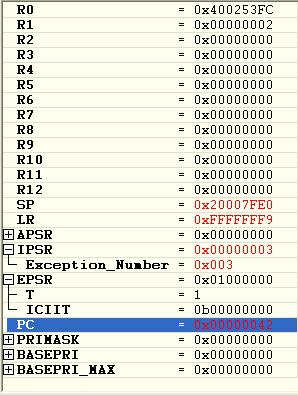
\includegraphics[scale=0.7]{img/411-register-trimmed.png} \\
\small{Figure 2: Status of the registers after the hard fault.}
\end{center}

\paragraph{}
In the next portion of the lab, we created a HardFault Handler. For the first part of this portion, we compared the vector table of our code, to the vector table found in the documentation. We found that the \emph{Stack Pointer}, \emph{Reset}, and \emph{Bus Fault} all corresponded to the documentation. 

\begin{center}
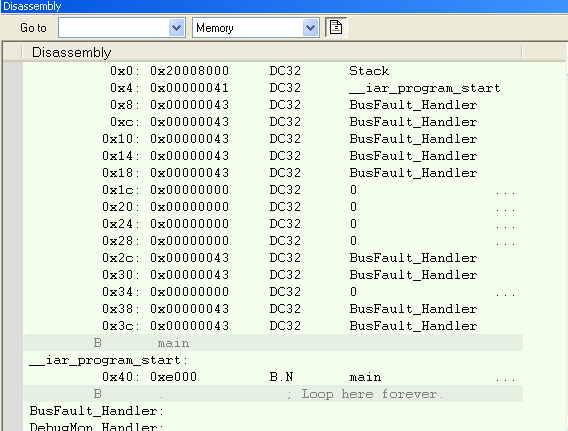
\includegraphics[scale=0.7]{img/421-diassembly.png} \\
\small{Figure 3: Vector table found in our program. Note 0x0, 0x4, \& 0x14}
\end{center}

\paragraph{}
Next we edited the code to add a hard fault handler. This simply captured a hard fault, and sent it into an infinite loop. In a real system, I think you would have this manage the fault, perhaps display an error code, I wonder if a Windows BSOD is an example of this. After we ran the code with this modified handler, we found that the handler was then executed when the program caused the hard fault. We also found that the vector table was closer to that which was specified in the documentation. That is, the \emph{Stack Pointer}, \emph{Reset}, \emph{Bus Fault}, and now the \emph{HardFault} all corresponded to the documentation. 

\paragraph{}
For the final experiment, we enabled Mode Clock Gating. To do this, we needed to inspect page 340 of the TI documentation. Note the figure below. According to the documentation, to enable mode clock gating, we needed to set the 6th bit in a certain register to 1. This was accomplished with the following assembly command: \emph{MOVS    R1, \#0x20}. Note, \emph{0x20 = 00100000}.

\begin{center}
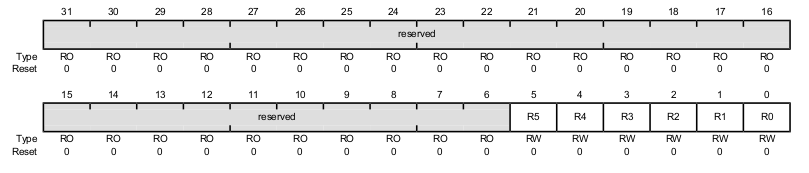
\includegraphics[scale=0.5]{img/mcg.png} \\
\small{Figure 4: Clock Mode Gating diagram}
\end{center}

\paragraph{}
Since the instructions now set mode clock gating, the \emph{STR     R1, [R0]} code segment no longer caused a hard fault. It successfully went through the \emph{CauseMemFault} branch, and returned to the main, where it then looped forever. 

\paragraph{}
I had a much easier time comprehending this lab than the 1st. I definitely have a better understanding of register manipulation, monitoring system faults, and their relation to the vector table. 

\end{document}